\section{Transport Construction}
\label{sec:transport}

Let $C(D)$ denote the set of chamber states.

\subsection{Transport Moves}

Define
\[
T_1 = FV, \qquad T_2 = VF.
\]

\subsection{Definition of the Graph}

\begin{definition}[Thalean graph]

The graph $G_{60}$ has vertex set $C(D)$.

Two vertices are adjacent if one is obtained from the other by
applying $T_1$ or $T_2$ (or their inverses).

\end{definition}

\begin{proposition}

The graph $G_{60}$ is $4$-regular.

\end{proposition}

\begin{proof}

From any chamber state $x$, the transport moves $T_1$ and $T_2$
produce two adjacent chamber states.

Since these moves are invertible, the inverse transformations
$T_1^{-1}$ and $T_2^{-1}$ produce two additional adjacent states.

These four transformations yield four distinct adjacent vertices.
Distinctness follows from the geometry of the transport moves,
which move the chamber state to different edges of the
dodecahedron.  This can also be verified directly from the
explicit adjacency data provided in Appendix~B.

\end{proof}

\begin{figure}[h]
\centering
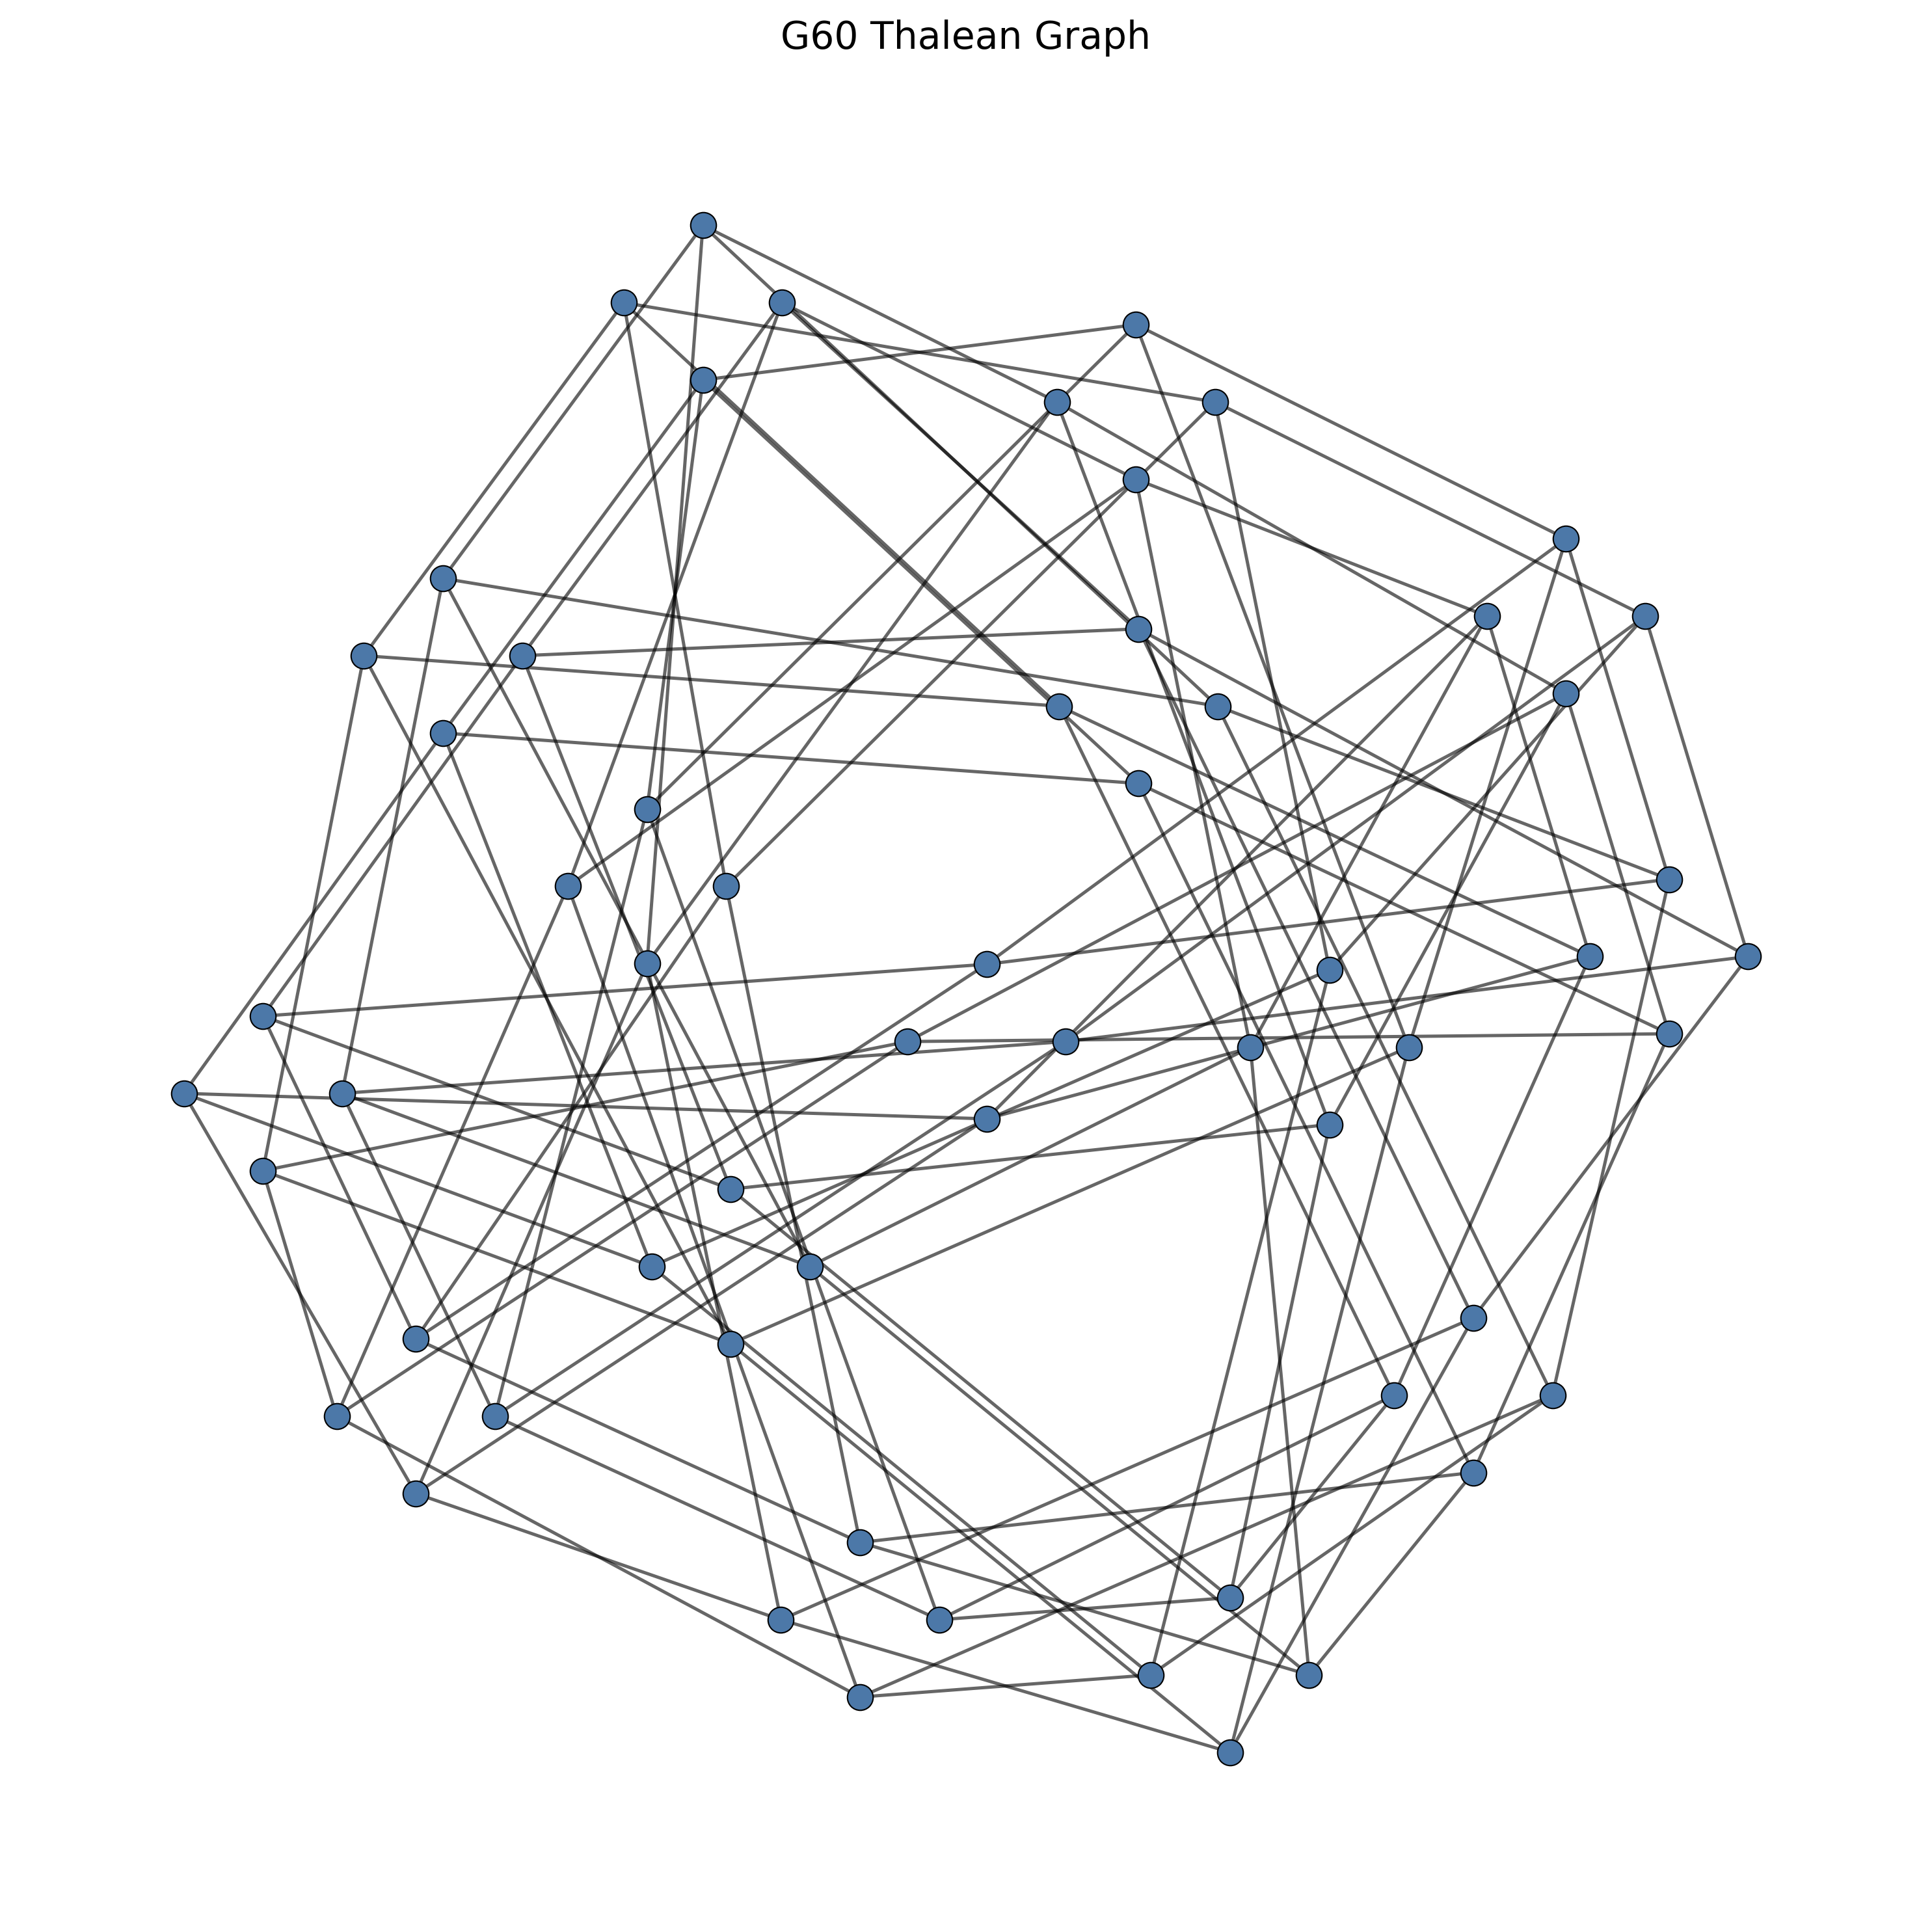
\includegraphics[width=0.72\textwidth]{figures/g60_graph.png}
\caption{Visualization of the graph $G_{60}$.}
\end{figure}

Thus

\[
|V(G_{60})| = 60,\qquad |E(G_{60})| = 120.
\]

